\chapter{Aufgabenanalyse}
\section{Beschreibung Eingabedatei}

Die Eingabedatei muss UTF-8-kodiert sein;
anderenfalls wird eine Exception mit der Meldung „Eingabedatei ist nicht UTF-8 kodiert“ ausgelöst.
Die Datei gliedert sich in exakt drei Abschnitte: Zeitraum:, Einfallspunkte: und Kreuzungen:.
Jeder Abschnitt darf höchstens einmal vorkommen – doppelte Abschnitte führen zu einem Abbruch mit einer spezifischen Fehlermeldung.

Im Abschnitt Zeitraum: werden zwei Parameter erwartet: die Gesamtdauer der Simulation in Sekunden (maxTime) sowie die Taktfrequenz (clockrate),
also das Intervall in Sekunden, in dem Fahrzeuge generiert werden.
Beide Werte müssen positive Ganzzahlen sein. maxTime darf dabei 24 Stunden (86.400 Sekunden) nicht überschreiten.
Ein Eintrag wie z.,B. „50.0“ würde eine Fehlermeldung hervorrufen,
da Dezimalzahlen nicht erlaubt sind. Auch muss clockrate kleiner oder gleich maxTime sein.

Der Abschnitt Einfallspunkte: definiert Punkte,
an denen Fahrzeuge in das System eintreten.
Jede Zeile folgt dem Format Name X Y Ziel Takt. 
abei dürfen Namen maximal 100 Zeichen lang sein und nicht doppelt vorkommen.
Die Koordinaten X und Y müssen Gleitkommazahlen im Bereich von -1000 bis +1000 sein.
Zudem wird geprüft, dass kein Punkt näher als 0{,}1 Einheiten (entspricht 10 Metern) zu einem bereits definierten Punkt liegt.
Als Ziel wird eine Kreuzung angegeben, zu der das erste Fahrzeug weitergeleitet wird.
Der Takt bestimmt die Häufigkeit der Fahrzeuggenerierung in Sekunden und muss eine positive ganze Zahl sein.

Im Abschnitt Kreuzungen: wird jede Zeile im Format Name X Y Ziel1 Anteil1 Ziel2 Anteil2 ... erwartet.
Auch hier sind Namen auf 100 Zeichen begrenzt und dürfen nicht mehrfach vorkommen.
Die Ziel-Anteil-Paare müssen mindestens zweimal vorkommen,
wobei die Anzahl der Teile ungerade sein muss (wegen Name, X und Y zu Beginn).
Der Anteil (relative Wahrscheinlichkeit) muss als Dezimalzahl mit Punkt angegeben sein und zwischen $10^6$ und $10^{-6}$ liegen.
Auch hier dürfen Koordinaten nicht zu nahe beieinanderliegen.

Orte dürfen nicht gleichzeitig Einfallspunkte und Kreuzungen sein. Zudem müssen alle in Einfallspunkten oder Kreuzungen genannten Zielorte tatsächlich existieren – entweder als Kreuzung oder als anderer Einfallspunkt.

% \begin{figure}[h!]
%     \centering
%     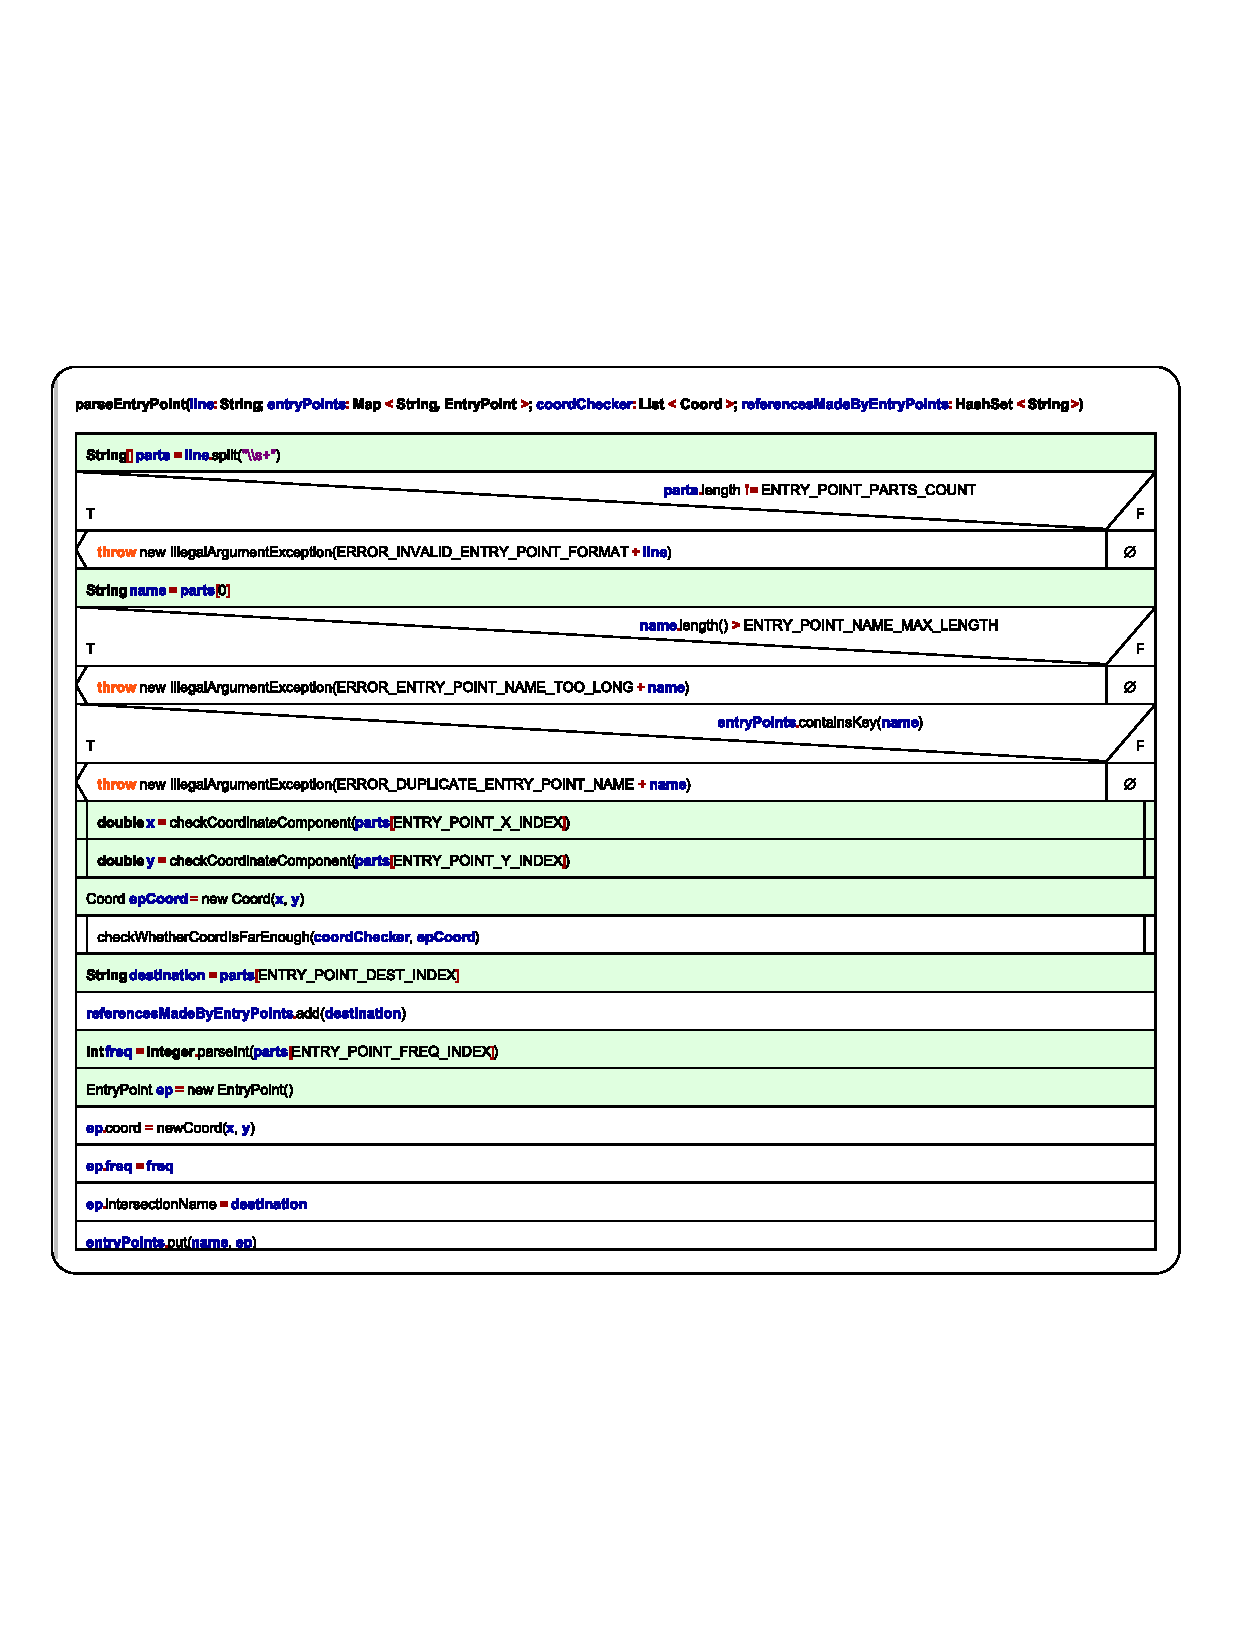
\includegraphics[width=0.8\textwidth]{nassis/TextFileReader/parseEntryPoint-4.pdf}
%     \caption{Example caption}
%     \label{fig:example}
% \end{figure}
